\subsection{三角函数}

若把（定义在 A 上的）函数 \(\cos\theta\) 、\(\sin\theta\) 、\(\tan\theta\) 、\(\cot\theta\) 与 R 到 A 上的同态 \(x\to\Im(x/a)\) 复合，则如此得到的函数

\[
\cos \Im \left(\frac {x}{a}\right), \quad \sin \Im \left(\frac {x}{a}\right), \quad \tan \Im \left(\frac {x}{a}\right), \quad \cot \Im \left(\frac {x}{a}\right)
\]

分别称为数 \(x\) 相对于底 \(a\) 的余弦、正弦、正切与余切，并记作 \(\cos_a x\) 、\(\sin_a x\) 、\(\tan_a x\) 、\(\cot_a x\) 。映射 \(x \to \cos_a x + i \sin_a x\) 是 \(\theta \to \cos \theta + i \sin \theta\) 与 \(x \to \Im(x/a)\) 的复合，因而由第 2 号中 \(\cos \theta\) 与 \(\sin \theta\) 的定义，我们有恒等式

\[
e \left(\frac {x}{a}\right) = \cos_ {a} x + i \sin_ {a} x,\tag{5}
\]

它等价于

\[
\cos_ {a} x = \Re \left(e \left(\frac {x}{a}\right)\right), \quad \sin_ {a} x = \Im \left(e \left(\frac {x}{a}\right)\right),
\]

并且由 (4)，它也等价于

\[
\cos_ {a} x = \frac {\mathrm{I}}{2} \left(e \left(\frac {x}{a}\right) + e \left(- \frac {x}{a}\right)\right), \quad \sin_ {a} x = \frac {\mathrm{I}}{2 i} \left(e \left(\frac {x}{a}\right) - e \left(- \frac {x}{a}\right)\right).
\]

由此得到恒等式

\[
\cos_ {b} x = \cos_ {a} \left(\frac {a x}{b}\right), \quad \sin_ {b} x = \sin_ {a} \left(\frac {a x}{b}\right).\tag{6}
\]

在不涉及数值计算的数学分支中所出现的三角函数，只有上述相对于基 \(2\pi\) 的那些函数；这些函数简单地记作 \(\cos x\) 、\(\sin x\) 、\(\tan x\) 、\(\cot x\) ，以代替 \(\cos_{2\pi}x\) 、\(\sin_{2\pi}x\) 、\(\tan_{2\pi}x\) 、\(\cot_{2\pi}x\) 。出于数值计算的目的，有对应于基 a = 360 与 a = 400 的三角函数表；而公式 (6) 使我们能推出相对于任何其他基的三角函数的值。

前面回忆过的角的余弦与正弦之间的关系，显然给出度量这些角的数之间的同样的关系；特别地，我们有

\[
\begin{array}{r l} & {\cos_ {a} (x + y) = \cos_ {a} x \cos_ {a} y - \sin_ {a} x \sin_ {a} y,} \\ & {\sin_ {a} (x + y) = \sin_ {a} x \cos_ {a} y + \sin_ {a} y \cos_ {a} x,} \\ & {\cos_ {a} (- x) = \cos_ {a} x, \qquad \sin_ {a} (- x) = - \sin_ {a} x,} \\ & {\qquad \cos_ {a} ^ {2} x + \sin_ {a} ^ {2} x = 1.} \end{array}
\]

函数 \(\cos_{a}x\) 与 \(\sin_{a}x\) 在 R 上连续，并且以 a 为周期；此外，a 是这些函数的基本周期，因为关系 \(\cos_{a}x = \cos_{a}y\) 蕴含或者 \(\sin_{a}x = \sin_{a}y\) ，或者

\[
\sin_ {a} x = - \sin_ {a} y, \quad \text { i.e., }
\]

\[
e \left(\frac {x}{a}\right) = e \left(\frac {y}{a}\right) \quad \text { or } \quad e \left(\frac {x}{a}\right) = e \left(- \frac {y}{a}\right),
\]

从而或者

\[
x \equiv y (\mathrm{mod} a) \quad \text { or } \quad x \equiv - y (\mathrm{mod} a);
\]

而类似地，

\[
\sin_ {a} x = \sin_ {a} y
\]

等价于 \(x \equiv y \pmod{a}\) 或者 \(x + y \equiv \frac{1}{2} a \pmod{a}\) 。

由此可知，\(\cos_{a}x\) 在区间 \([0,\frac{1}{2}a]\) 中绝不两次取同一个值；因此，当限制在这个区间上时，它是该区间到区间 \([-1,+1]\) 上的一个双射映射。由于 \(\cos_{a}0=1\) 且 \(\cos_{a}\left(\frac{1}{2}a\right)=-1\) ，故 \(x\to\cos_{a}x\) 是 \([0,\frac{1}{2}a]\) 到 \([-1,1]\) 上的一个严格递减映射（第四章，§ 2，第 6 号，定理 5 及其注）。\(\cos_{a}x=0\) （当 x=a/4），\(\cos_{a}x>0\) 对 \(0\leqslant x<a/4\) 成立，\(\cos_{a}x<0\) 对 \(a/4<x\leqslant a/2\) 成立。由 \(\cos_{a}(-x)=\cos_{a}x\) 可以推出 \(\cos_{a}x\) 在区间 \([-\frac{1}{2}a,0]\) 中的变化情况，从而由周期性推出它在整个 R 上的变化情况（图 8）。由 \(\sin_{a}x=-\cos_{a}(x+a/4)\) 又可推出 \(\sin_{a}x\) 在 R 中的变化情况（图 8）。

\pandocbounded{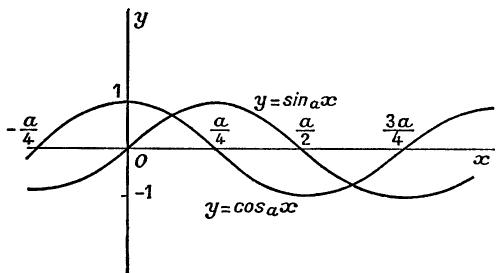
\includegraphics[keepaspectratio]{images/part001_7529c0a8.jpg}}\\
图 8.

函数 \(\tan_{a}x\) 是 \(\mathbf{R}\) 到 \(\tilde{\mathbf{R}}\) 上的一个连续映射；它取值 \(\infty\) 于诸值 \(\frac{1}{4} a + \frac{1}{2} ka\) 处（ \(k \in \mathbf{Z}\) ）。由于 \(\frac{1}{2} a\) 是 \(\tan_{a}x\) 的一个周期，故它是一个基本周期。在区间 \([0, \frac{1}{4} a]\) 中，\(\sin_{a}x\) 从 \(0\) 递增到 \(1\) ，\(\cos_{a}x\) 从 \(1\) 递减到 \(0\) ，因此 \(\tan_{a}x\) 在 \([0, \frac{1}{4} a[\) 中严格递增，并把这个区间映射到 \([0, +\infty[\) 上；由此推出 \(\tan_{a}x\) 在区间 \(]-\frac{1}{4}a,+\frac{1}{4}a[.\) 中严格递增，并且是这个区间到 R 上的一个同胚（图 9）。

\pandocbounded{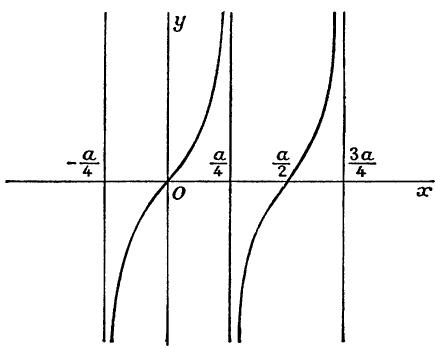
\includegraphics[keepaspectratio]{images/part001_329f289a.jpg}}\\
图 9.

